%% Information Sciences / Elsevier CAS manuscript package.
%% SC-FMA manuscript for Knowledge Engineering and Audit Prioritization
\documentclass[a4paper,fleqn]{cas-sc}

\usepackage[numbers,sort&compress]{natbib}
\usepackage{amsmath}
\usepackage{amssymb}
\usepackage{booktabs}
\usepackage{array}
\usepackage{graphicx}
\usepackage{xurl}
\usepackage{amsthm}
\newtheorem{theorem}{Theorem}[section]
\newtheorem{lemma}[theorem]{Lemma}
\newtheorem{corollary}[theorem]{Corollary}
\usepackage{algorithm}
\usepackage{algpseudocode}
\usepackage{multirow}
\usepackage{makecell}
\usepackage{placeins}
\usepackage{CJKutf8}
\usepackage{hyperref}
\hypersetup{colorlinks=true,linkcolor=blue,citecolor=blue,urlcolor=blue}
\newcolumntype{Z}[1]{>{\raggedright\arraybackslash}p{#1}}
\newcommand{\wstruct}{\ensuremath{\mathbf{w}_{\mathrm{struct}}}}

\begin{document}
\let\WriteBookmarks\relax
\def\floatpagepagefraction{1}
\def\textpagefraction{.001}
\pagenumbering{arabic}

\shorttitle{Structurally-Calibrated Functional Metacognitive Attribution}
\shortauthors{Ma and Wang}

\title[mode=title]{Structurally-Calibrated Functional Metacognitive Attribution for Audit Prioritization in Knowledge-Intensive Reasoning}

\author[1]{Haoran Ma}
\ead{mahaoran0000@foxmail.com}

\author[1,2]{Ningning Wang\corref{cor1}}
\ead{wangningning@bistu.edu.cn}

\cortext[cor1]{Corresponding author.}
\renewcommand{\printorcid}{}

\affiliation[1]{organization={College of Management Science and Engineering, Beijing Information Science and Technology University},
            city={Beijing},
            postcode={102200},
            country={China}}

\affiliation[2]{organization={Institute of Information Systems, ESG Intelligent Application Innovation Research Center},
            city={Beijing},
            postcode={102200},
            country={China}}

\begin{abstract}
Knowledge-intensive information systems expose process annotations, retrieval checks, entity bindings, graph nodes, and verification records. Curators often inspect these artifacts under fixed audit budgets and need records that show supplied annotation fidelity, dependency, redundancy, bottleneck exposure, and diagnostic role. We introduce Structurally-Calibrated Functional Metacognitive Attribution (SC-FMA), where ``metacognitive'' is used operationally for engineering inspection of observable process artifacts. SC-FMA represents artifacts as dependency-aware audit graphs and uses the Structurally-Calibrated Utility (SCU) objective as a representation constraint system. The central real-data finding is a boundary rather than a ranking gain: on a locked PRM800K-derived process-annotation distribution (4,417 samples; 34,219 labeled artifacts), the supervised \wstruct{} fidelity field remains strongest (Spearman $\rho=0.611$), Ridge tracks it with a small loss ($\rho=0.604$), and QP ($\rho=0.442$) and Projection ($\rho=-0.135$) are lower. Structural necessity alone is anti-correlated with PRM800K labels ($\rho=-0.418$), and QP degrades on long traces, so the current graph signal is treated as a diagnostic interface rather than an independently validated ranking signal. Rule-derived audit-target retrieval shows that raw fields recover much of the target signal; SC-FMA adds organization for redundancy and structural-overcorrection cases, while bottleneck protection is QP-derived internal consistency. Countries-KG and synthetic stress tests are backend and implementation diagnostics. The evidence supports a bounded audit-record representation layer; human audit usefulness, production knowledge-base validation, same-supervision structure-only baselines, and cross-domain transfer remain future work.
\end{abstract}

\begin{keywords}
knowledge engineering \sep knowledge representation \sep maintenance-oriented knowledge analysis \sep knowledge graphs \sep audit prioritization \sep representation-aware attribution
\end{keywords}

\maketitle

\section{Introduction}

Knowledge-intensive information systems increasingly expose intermediate artifacts during retrieval, annotation, validation, update, and reuse. These artifacts include graph nodes, entity bindings, verification records, rule-like operations, retrieval checks, process annotations, and reasoning traces. Once exposed, they become knowledge artifacts that must be represented, organized, curated, and reused across the knowledge lifecycle. The challenge is that these artifacts are heterogeneous, uncertain, and often more numerous than the audit capacity available to curators.

Existing methods supply useful signals for this setting. Process-annotation methods attach scalar quality estimates to intermediate artifacts. Local utility-signal methods estimate artifact influence. Graph-based salience methods identify structurally prominent nodes. Fixed-budget audit also needs a reusable record that combines these signals with dependency structure and diagnostic interpretation. Such a record helps curators see whether an artifact provides local evidence, supports a dependency, duplicates earlier support, or exposes a downstream bottleneck.

This paper introduces Structurally-Calibrated Functional Metacognitive Attribution (SC-FMA) as a knowledge representation transformation layer for this setting. In SC-FMA, ``metacognitive'' is used operationally. It names engineered secondary inspection of observable attribution-related artifacts through structural and functional decomposition; it is not a claim about latent cognitive-state monitoring. Readers can equivalently read the method as structurally calibrated functional attribution over observable process artifacts. SC-FMA transforms intermediate knowledge artifacts into structured audit records. It represents their dependencies, calibrates supplied annotation or utility signals, and attaches audit reasons and diagnostic interpretations. Audit priority is one field within this record.

SC-FMA organizes fixed-budget audit around a structured record. Process-annotation studies provide artifact-level fidelity signals~\cite{lightman2023verify,uesato2022solving}. Network and graph-explanation methods show why structural position, redundancy, and bottleneck exposure can matter~\cite{albert2000error,newman2010networks,ying2019gnnexplainer}. Simplex projection provides a familiar way to impose a fixed review budget~\cite{wang2013projection}. SC-FMA combines these ingredients as record fields: fidelity, structure, redundancy, bottleneck protection, and budget consistency.

The paper makes three contributions. First, it formulates fixed-budget audit-record construction for structured knowledge artifacts. Second, it introduces SC-FMA and the SCU objective, which combine annotation fidelity, structural dependency, redundancy, and bottleneck roles into decomposed audit records. Third, it evaluates the representation on a PRM800K process-annotation dataset, a Countries-KG backend feasibility study, rule-derived audit-target retrieval, and controlled synthetic calibration.

The main findings follow the same knowledge-engineering workflow, with a negative result at the center of the real-data route. On the PRM800K process-annotation dataset, \wstruct{} is treated as a supervised fidelity field for artifact records and remains the strongest real-data ranking field. Under the frozen hash split (4,417 samples and 34,219 labeled artifacts), SC-FMA Ridge closely tracks \wstruct{} (Spearman $\rho = 0.604$ versus $0.611$) while exposing decomposition fields; QP and Projection are lower-consistency diagnostic variants on this strong-fidelity route, and QP degrades most strongly on long traces. The Countries-KG backend feasibility study shows that typed ontology edges can change structural-dependency representation at the graph interface, but this sensitivity is also a reliability warning for the structural-necessity signal. Rule-derived audit-target retrieval provides a field-level diagnostic of weak utility anchors, redundancy, and structural over-correction, plus a QP-derived bottleneck consistency check; a raw-field control separates field exposure from SCU joint optimization. Controlled synthetic calibration and ablation explain implementation behavior when labels explicitly encode structural preferences, not external audit value.

The remainder of this paper is organized as follows. Section~\ref{sec:related-work} reviews attribution, step-level annotation signals, graph-based knowledge engineering, and audit methods. Section~\ref{sec:methods} presents SC-FMA, the SCU objective, and its representation properties. Section~\ref{sec:experimental-results} reports diagnostics from real annotation evidence, knowledge-graph backend feasibility, and controlled calibration. Section~\ref{sec:discussion} interprets the method in the knowledge lifecycle. Section~\ref{sec:conclusions} concludes.

Figure~\ref{fig:overall-framework} gives the high-level knowledge-engineering workflow. SC-FMA sits between raw knowledge artifacts and potential review workflows: it represents artifacts as dependency graphs, calibrates annotation signals with SCU, and returns knowledge audit records with explicit structural roles and diagnostic interpretations.

\begin{figure}[pos=ht]
\centering

\includegraphics[width=\linewidth]{figures/fig_overall_framework.pdf}
\caption{Knowledge engineering workflow for SC-FMA. The figure should be read as a transformation from Knowledge Artifact $\rightarrow$ Representation $\rightarrow$ Graph Structure $\rightarrow$ SCU $\rightarrow$ Audit Record $\rightarrow$ Knowledge Curation. Raw reasoning traces, graph nodes, and process annotations are first organized as auditable knowledge artifacts, then represented through dependency-aware graph structure. SCU constructs structured audit records by preserving annotation or utility fidelity while adding structural dependency, redundancy, bottleneck, audit-reason, and diagnostic-interpretation fields. The resulting records support fixed-budget audit representation and diagnostic analysis; the audit-priority field is only a downstream use of the audit representation.}
\label{fig:overall-framework}
\end{figure}

\section{Related Work}
\label{sec:related-work}

\subsection{Attribution and Explanation}

Attribution methods ask which parts of an input, computation, or structure matter for a decision. Integrated Gradients~\cite{sundararajan2017axiomatic}, SHAP~\cite{lundberg2017unified}, and LIME~\cite{ribeiro2016lime} return feature-level or local explanation signals, while ERASER evaluates extractive rationales~\cite{deyoung2020eraser}.

Structure-aware attribution adds graph context. Network studies show that importance can be non-local, redundant, or concentrated around bottleneck nodes~\cite{albert2000error,newman2010networks}; GNNExplainer selects compact explanatory subgraphs~\cite{ying2019gnnexplainer}. Human-centered XAI further shows that explanations must fit review tasks and organizational routines~\cite{miller2019explanation,arrieta2020explainable,amershi2019guidelines,kaplan2024xai}.

These lines motivate the audit-triage setting. Salience identifies important evidence; audit triage additionally needs role labels for local support, duplicated evidence, downstream dependencies, and weak upstream signals. Entailment-tree and counterfactual methods add intermediate or contrastive evidence~\cite{dalvi2021entailmenttrees,wijekoon2023counterfactual}; SC-FMA keeps the audit roles separate.

\subsection{Process Supervision and Process Reward Models}

Process supervision assigns annotation signals to intermediate artifacts as well as final answers. PRM800K showed that per-artifact human labels can support verifier-guided best-of-$N$ search relative to outcome reward models~\cite{lightman2023verify}; GSM8K made this verifier setting concrete~\cite{cobbe2021training}. Process-based feedback also reduced reasoning errors when outcome success appeared saturated~\cite{uesato2022solving}. These studies provide the artifact-resolved fidelity signal that SC-FMA calibrates.

A parallel line makes verification, critique, and revision available as process units. Chain-of-thought and self-consistency expose sampled reasoning paths~\cite{wei2022cot,wang2022selfconsistency}. Tree of Thoughts and ReAct add search or action structure~\cite{yao2023tot,yao2022react}, while Reflexion and Self-Refine turn revision steps into supervision targets~\cite{shinn2023reflexion,madaan2023selfrefine}.

Recent process-diagnostic resources also show that step-level signals need distributional checks. Math-Shepherd studies automatic step verification without human annotations~\cite{wang2024mathshepherd}, and ProcessBench evaluates process-error identification across models~\cite{zheng2024processbench}. These resources help assess scalar step signals, which SC-FMA uses as inputs to structural calibration.

\subsection{Graph-Based Knowledge Engineering and Audit Methods}

Graph-based knowledge engineering shows how structured intermediate states can be made inspectable. Knowledge-engineering methods have long treated representation, inference, and maintenance-oriented review as coupled design problems~\cite{studer1998knowledge}. Early expert systems such as MYCIN and DENDRAL demonstrated the value of structured knowledge representation~\cite{buchanan1984mycin,lindsay1980dendral}. Cognitive architectures such as Soar and ACT-R also made internal states and operator applications available for step-level review~\cite{laird2012soar,anderson2004actr}. In information systems, related work on knowledge management and algorithmic accountability emphasizes that AI artifacts must be represented in ways that support transparency, traceability, and organizational oversight~\cite{dwivedi2021artificial,raji2020closing}.

Modern knowledge-intensive pipelines connect language models with structured knowledge. Knowledge graphs provide a representation substrate for entities, relations, constraints, and quality signals~\cite{hogan2021knowledge}. RAG and GraphRAG expose passages, entity graphs, and community summaries as evidence~\cite{lewis2020rag,gao2023ragsurvey,edge2024graphrag}. KG-RAG, knowledge-enhanced language models, and LLM-KG integration expose entity links, triples, and relation paths as reviewable artifacts~\cite{sanmartin2024kgrag,hu2024knowledgeenhanced,pan2024unifying}. Recent surveys and KG-quality studies show why graph-quality signals become part of the audit surface~\cite{yang2025kbllmsurvey,chen2025kgquality,dai2025llmkg}. Similar pressure appears in long-tail KG-augmented QA and engineering-design RAG, where sparse support and heterogeneous evidence make exhaustive review unrealistic~\cite{huang2025prompting,siddharth2024retrieval,liu2025knowledgereasoning}.

Across these settings, the challenge is no longer simply recovering intermediate evidence. Modern pipelines already expose passages, entity links, relation paths, and verification records. The harder question is how to allocate limited curation budget and preserve records for refinement, update, and reuse~\cite{paulheim2017knowledge,higgins2008dcc}. SC-FMA converts exposed artifacts into graph-aware audit records for that purpose.

\subsection{Summary of Research Gap}

Existing work supplies three ingredients: local attribution identifies salient evidence, process supervision supplies step-level annotation fidelity, and graph-based knowledge engineering exposes structural context. SC-FMA combines them into a representation layer that turns exposed knowledge artifacts into inspectable records for fixed-budget knowledge audit.

\subsection{Comparison with Alternative Representations}

The experimental comparisons below use internal scalar views and reproducible ablations aligned with the audit-record object. IG, SHAP, LIME, GNNExplainer, frozen PRM scorers, and related methods define neighboring objectives whose native outputs include feature attributions, local explanations, explanatory subgraphs, and scalar reward signals. SC-FMA targets a decomposed audit record with fidelity, structural dependency, redundancy, bottleneck, audit-reason, and diagnostic-interpretation fields.

\begin{table}[ht]
\caption{Output objects of neighboring explanation methods and SC-FMA. The table positions each method family by its native representation.}
\label{tab:alternative-representation-comparison}
\centering
\small
\renewcommand{\arraystretch}{1.08}
\begin{tabular}{Z{0.26\linewidth}Z{0.30\linewidth}Z{0.32\linewidth}}
\toprule
\textbf{Method family} & \textbf{Native output object} & \textbf{Relation to audit-record construction} \\
\midrule
IG, SHAP, LIME & Feature-level or local attribution scores & Provides salience signal. \\
GNNExplainer-style graph explanation & Compact explanatory subgraph & Provides structural subset. \\
Frozen PRM or process scorer & Scalar step or prefix signal & Provides fidelity field. \\
SC-FMA & Decomposed audit record & Constructs fidelity, dependency, redundancy, bottleneck, reason, and interpretation fields. \\
\bottomrule
\end{tabular}
\end{table}

\section{Method}
\label{sec:methods}

\subsection{Workflow Overview}

\textbf{Workflow statement.} SC-FMA takes exposed process artifacts through sequence normalization, graph construction, SCU calibration, and audit-record emission.

The input is a set of observable knowledge artifacts such as retrieval checks, entity bindings, rule-like operations, verification records, or reflective annotations. These artifacts are normalized into an auditable sequence, converted into a graph representation with temporal and optional domain edges, calibrated by SCU against the supplied annotation or utility signal, and emitted as audit records. The empirical study evaluates this record behavior with representation diagnostics.

\subsection{SC-FMA as a Representation Layer}

SC-FMA represents structural dependencies among intermediate knowledge artifacts and converts them into audit-oriented records. The records preserve fidelity information while adding structural role and diagnostic-interpretation fields.

\subsection{Formal Problem Definition}

\textbf{Input.} SC-FMA takes an observable artifact sequence $T=(s_1,\ldots,s_k)$, where each unit $s_i$ may be a verification, reflection, retrieval, entity-binding, or rule-like operation available for audit. The sequence is converted into a graph $G=(V,E)$ whose nodes correspond to artifact units and whose edges encode temporal adjacency plus optional topical or domain-specific relations. The method also receives a utility or fidelity signal $u$ over the same units. This signal may come from local utility estimation, a proxy representation signal, or a learned step-annotation model, and SC-FMA treats it as the fidelity signal to be preserved when it is informative.

\textbf{Output and objective.} The output is a set of calibrated knowledge artifact records. Each record contains an audit-priority field plus fidelity, structural-dependency, redundancy, bottleneck, audit-reason, and diagnostic-interpretation fields. The objective is to preserve useful utility signal, incorporate observable artifact structure, and attach each selected artifact to an interpretable audit-oriented analysis.

\subsection{SCU Objective and Audit Decomposition}
\label{sec:scu-objective}

SCU is a representation constraint system for fixed-budget audit records. It tracks an informative fidelity input when available while making the structural reason for each priority visible. Dependency, redundancy, and bottleneck fields indicate whether a selected artifact is local evidence, dependency support, repeated support, or a later-artifact dependency.

For an artifact sequence with $k$ auditable units, let $\tilde{\mathbf{c}}\in\mathbb{R}^k$ denote the normalized utility or proxy-fidelity input. In the locked PRM800K process-annotation stage, \wstruct{} denotes the frozen Ridge regressor used as this fidelity signal. In the binary-correctness diagnostic setting, $\tilde{\mathbf{c}}$ is a coarse sequence-level local utility anchor: it records how an observed outcome changes under a documented intervention. Let $\tilde{\mathbf{n}}$ denote normalized structural necessity from graph perturbation diagnostics, $\mathbf{R}$ a redundancy matrix, and $\mathbf{b}$ a bottleneck indicator. The main notation is summarized in Table~\ref{tab:notation}.

\begin{table}[ht]
\caption{Notation used by the SCU objective and audit-record fields.}
\label{tab:notation}
\centering
\small
\renewcommand{\arraystretch}{1.08}
\begin{tabular}{Z{0.18\linewidth}Z{0.70\linewidth}}
\toprule
\textbf{Symbol} & \textbf{Meaning in this paper} \\
\midrule
$\tilde{\mathbf{c}}$ / \wstruct{} & Normalized fidelity input; in the locked PRM800K stage, \wstruct{} is the dev-trained frozen Ridge fidelity signal. \\
$\tilde{\mathbf{n}}$ & Normalized structural-necessity input from graph perturbation diagnostics. \\
$\mathbf{R}$ & Redundancy matrix over auditable artifact units. \\
$\mathbf{b}$ & Bottleneck indicator vector. \\
$\mathbf{w}$ & Calibrated audit-priority field on the probability simplex. \\
$\alpha,\beta,\gamma,\delta$ & Fidelity, structural-necessity, redundancy, and bottleneck coefficients in SCU. \\
Ridge / QP / Projection & Preservation softmax, constrained SCU solver, and topology-constrained simplex projection variants. \\
\bottomrule
\end{tabular}
\end{table}

SC-FMA computes calibrated priority-field values $\mathbf{w}$ on the probability simplex
\begin{equation}
\mathcal{W}=\{\mathbf{w}\in\mathbb{R}_{+}^{k}: \sum_i w_i = 1\}
\label{eq:scu-feasible-set}
\end{equation}
by minimizing the SCU objective:
\begin{equation}
L(\mathbf{w}) =
\alpha\|\mathbf{w} - \tilde{\mathbf{c}}\|_2^2
+ \beta\|\mathbf{w} - \tilde{\mathbf{n}}\|_2^2
+ \gamma\,\mathbf{w}^{\top}\mathbf{R}\mathbf{w}
- \delta\sum_i b_i \log(w_i).
\label{eq:scu}
\end{equation}
Unless otherwise stated, $\alpha,\beta,\gamma,\delta \ge 0$ and the symmetric part of $\mathbf{R}$ is treated as positive semidefinite on the simplex tangent subspace. The terms encode fidelity, structural alignment, redundancy regularization, and non-zero bottleneck regularization. The fidelity signal is dominant; redundancy and bottleneck terms mainly encourage interpretable decomposition fields under the current validation setting. Detailed notation, construction rules, algorithms, and proofs are provided in the supplementary material.

\subsection{Artifact Representation}

Each artifact sequence is represented as an ordered set of auditable knowledge artifacts. The implementation supports units from structured reflection tags and free-text chain-of-thought segmentation. Segmentation is an observed input to the pipeline.

A node $v_i$ corresponds to one artifact unit. Temporal edges connect adjacent units, while topical edges connect units whose TF-IDF similarity exceeds the configured threshold. The graph serves as the representation substrate for knowledge dependencies. TF-IDF provides a lightweight fallback backend when richer domain relations are unavailable.

A supplementary graph-construction ablation replaces TF-IDF topical edges with Sentence-BERT embeddings (\texttt{sentence-transformers/all-MiniLM-L6-v2}, 384 dimensions). In that 800-trace fixture, the TF-IDF topical default (0.0515) did not exceed temporal-only edges (0.0596) on diagnostic structural-necessity consistency. The embedding backend (0.0615) was only slightly higher on the same readout.

These differences are too small to treat topical edges as a representation-field driver. We therefore read the graph layer as an interchangeable \emph{construction interface}. In this setting, the TF-IDF topology adds little annotation-order preservation value over the temporal chain and functions mainly as a fallback lexical cue; if the structural field is used for ranking rather than diagnostic record construction, this weak and sometimes negative alignment is a material limitation.

The graph constructor is modular. Semantic embeddings, entity links, knowledge graphs, ontologies, rule-dependency DAGs, and data-lineage graphs can replace the default without modifying SCU. The Countries-KG study (Section~\ref{sec:kg-pilot}) and the embedding ablation illustrate this interface.

\subsection{Structural Necessity, Redundancy, and Bottlenecks}

Structural necessity measures how much graph support is lost when a node is perturbed under a documented graph-level operation. The implementation uses PRUNE, CASCADE, and BYPASS diagnostics. PRUNE removes direct node support. CASCADE propagates disruption to downstream neighbors. BYPASS asks whether alternative paths can substitute for the removed artifact unit. The final necessity input $\tilde{\mathbf{n}}$ is the normalized summary of these observable graph diagnostics.

The redundancy matrix $\mathbf{R}$ captures pairwise similarity between artifact units. High redundancy means that two units appear to serve overlapping functions. The penalty $\mathbf{w}^{\top}\mathbf{R}\mathbf{w}$ discourages allocating large budget share to many mutually redundant units. In the current evidence package, this term records duplicated-audit pressure, but its direct contribution to annotation-order consistency is modest.

Bottleneck detection addresses the opposite pattern. Some nodes are not redundant, and their downstream exposure can make them worth inspecting even if the supplied fidelity signal is modest. The log-barrier prevents identified bottleneck nodes from receiving near-zero priority-field mass, keeping a possible single point of failure visible.

Figure~\ref{fig:local-utility-necessity} illustrates the local-utility--necessity mismatch. Figure~\ref{fig:variant-behavior} reports the three perturbation modes, and Figure~\ref{fig:resilience} shows the resilience curves. Together, the figures explain why the representation needs separate fidelity and structural fields: local utility, graph necessity, and resilience under removal capture related but distinct diagnostics.

\begin{figure}[pos=ht]
\centering
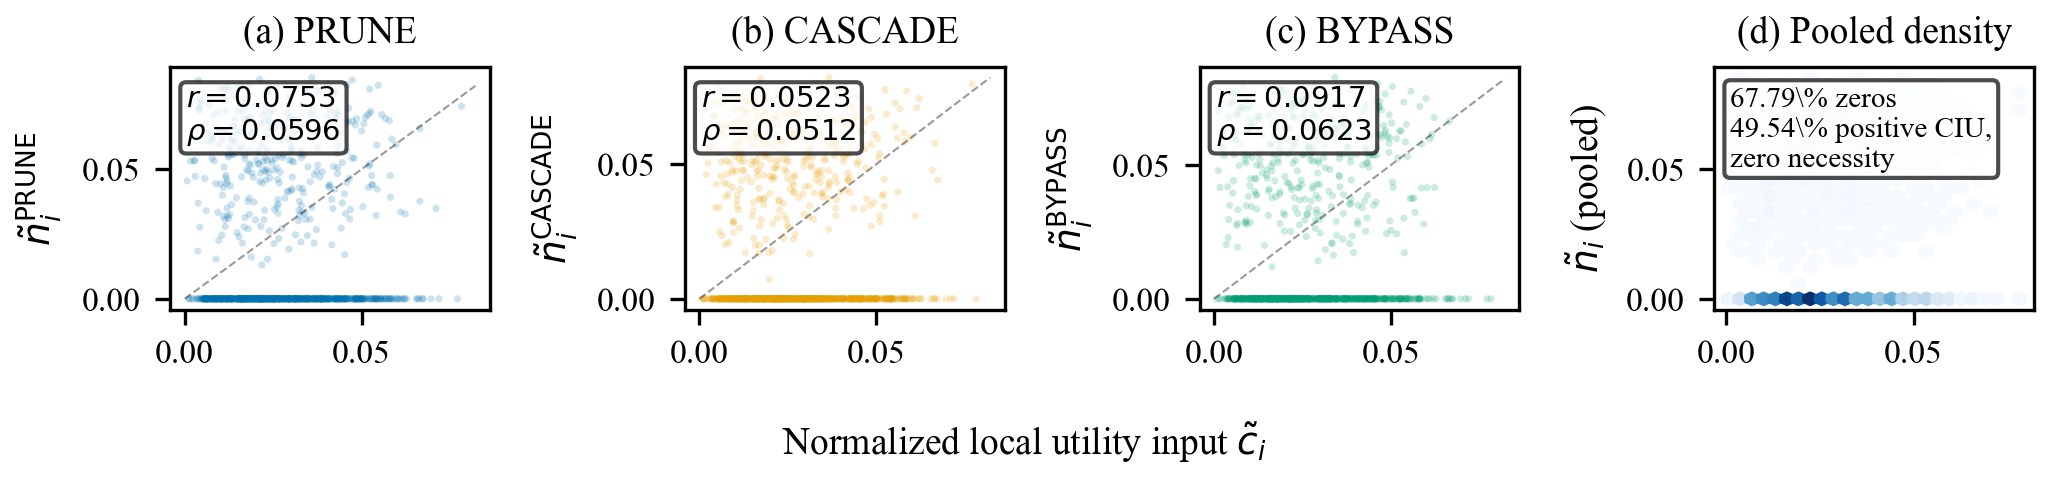
\includegraphics[width=\linewidth]{figures/fig_local_utility_necessity.png}
\caption{Structural diagnostic motivating calibration. Local utility and graph-level necessity diverge: many locally useful steps have low measured structural necessity, while some structurally exposed steps receive limited local utility signal. The shared $x$-axis $\tilde{c}_i$ denotes the normalized local utility input for step $i$. SC-FMA uses this mismatch as the reason for calibration.}
\label{fig:local-utility-necessity}
\end{figure}

\begin{figure}[pos=ht]
\centering
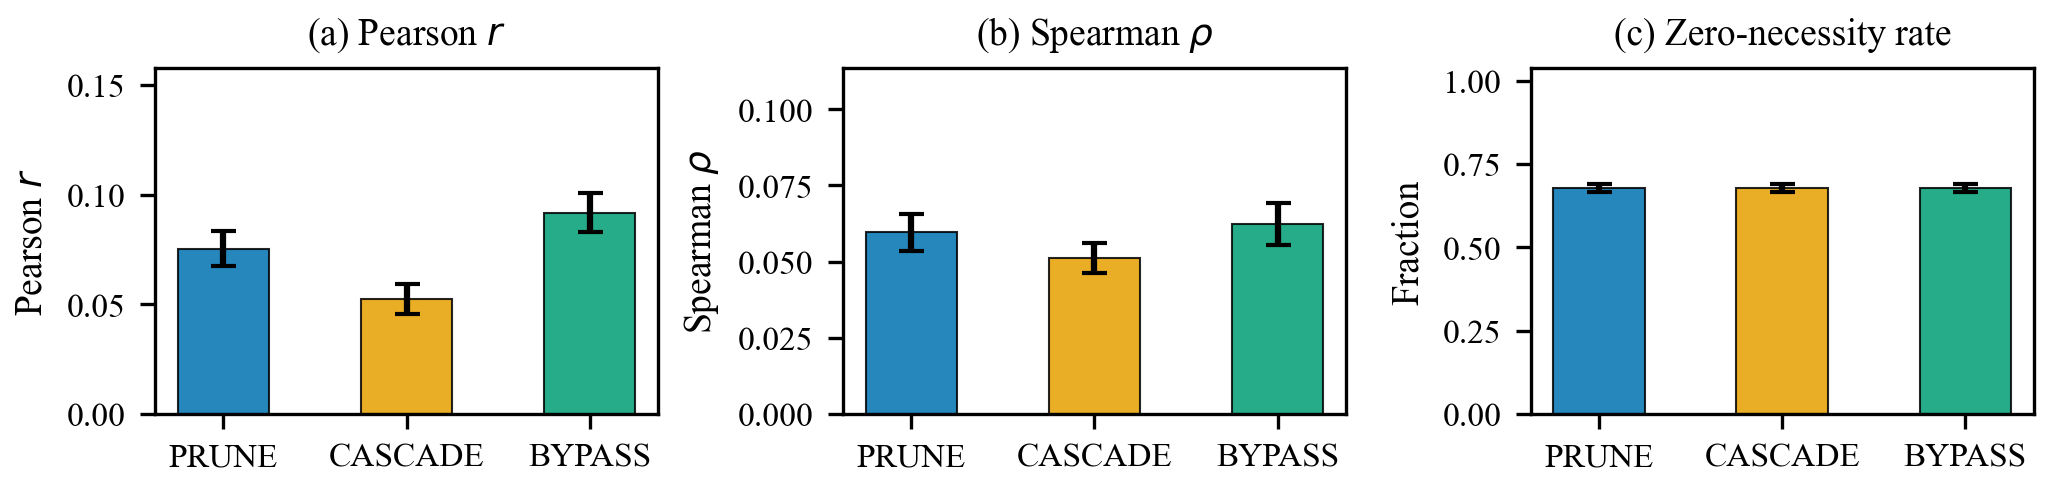
\includegraphics[width=\linewidth]{figures/fig_representation_variant_behavior.png}
\caption{Structural diagnostic summary by perturbation mode. The three perturbation modes (PRUNE, CASCADE, BYPASS) are reported with Pearson correlation, Spearman annotation-order consistency, and zero-necessity fraction. Error bars indicate 95\% bootstrap confidence intervals. The consistency across modes indicates that weak local-utility--necessity alignment persists across perturbation strategies.}
\label{fig:variant-behavior}
\end{figure}

Figure~\ref{fig:variant-behavior} keeps the perturbation evidence at the representation-diagnostic level. PRUNE, CASCADE, and BYPASS expose how structural necessity is measured under different graph operations; their role is to test whether the mismatch is stable enough to justify a separate structural field. The low and negative correlations also bound the reading of this signal: on lightweight lexical graphs for mathematical process annotations, structural necessity can be topology-sensitive or misaligned with human step labels and should be interpreted through graph-backend and perturbation diagnostics rather than as an independent quality metric.

\begin{theorem}[SCU well-posedness]
\label{thm:scu-well-posedness}
Let $\mathbf{R}_{s}=(\mathbf{R}+\mathbf{R}^{\top})/2$ and let $\mathcal{T}=\{\mathbf{z}\in\mathbb{R}^{k}:\mathbf{1}^{\top}\mathbf{z}=0\}$ be the tangent subspace of the simplex. Define the quadratic Hessian on this subspace as $\mathbf{H}_{q}=2((\alpha+\beta)\mathbf{I}+\gamma\mathbf{R}_{s})$. Assume $\alpha,\beta,\gamma,\delta \ge 0$ and $\mathbf{z}^{\top}\mathbf{R}_{s}\mathbf{z}\ge 0$ for every $\mathbf{z}\in\mathcal{T}$. Then the SCU objective in Eq.~\ref{eq:scu} is convex on the relative interior of the simplex in Eq.~\ref{eq:scu-feasible-set}. If $\mathbf{z}^{\top}\mathbf{H}_{q}\mathbf{z}>0$ for every nonzero $\mathbf{z}\in\mathcal{T}$, the quadratic part is strictly convex on the feasible subspace and the minimizer is unique. If $\delta>0$ and $b_i=1$, any finite minimizer assigns $w_i>0$ to that bottleneck node; the barrier therefore gives an interior guarantee for active bottleneck support. For non-redundant artifact-unit pairs with identical redundancy profiles and inputs ordered in the same direction, $\tilde c_i\ge \tilde c_j$ and $\tilde n_i\ge \tilde n_j$, the two-input priority-field relation is monotone before redundancy-induced redistribution. Once redundancy profiles differ, this monotonicity remains a local diagnostic property.
\end{theorem}

The theorem is a well-posedness check for the constrained representation program, not a source of empirical validation. Its monotonicity statement applies before redundancy-induced redistribution under matched redundancy profiles; the empirical sections therefore determine when the optimizer is useful or brittle.

We implement three variants of the same calibration procedure; they are not competing claims that one optimizer is universally best. SC-FMA Ridge uses a closed-form softmax over a linear combination of $\tilde{\mathbf{c}}$ and $\tilde{\mathbf{n}}$ and does not contain the $\gamma\mathbf{w}^{\top}\mathbf{R}\mathbf{w}$ redundancy term or the bottleneck log-barrier term. SC-FMA QP solves the full constrained program with redundancy and bottleneck terms. SC-FMA Projection applies a fast topology-constrained simplex projection onto the probability simplex~\cite{wang2013projection}. The validation sections report where each variant is appropriate.

The calibrated priority field is inspectable. For each selected artifact unit, the implementation can report whether the priority was driven mainly by fidelity, structural dependency, redundancy, or bottleneck regularization. The simplex constraint represents an audit budget: increasing one unit's priority decreases another unit's share. The output is a fixed-budget audit record with structured diagnostic fields.

\begin{figure}[pos=ht]
\centering
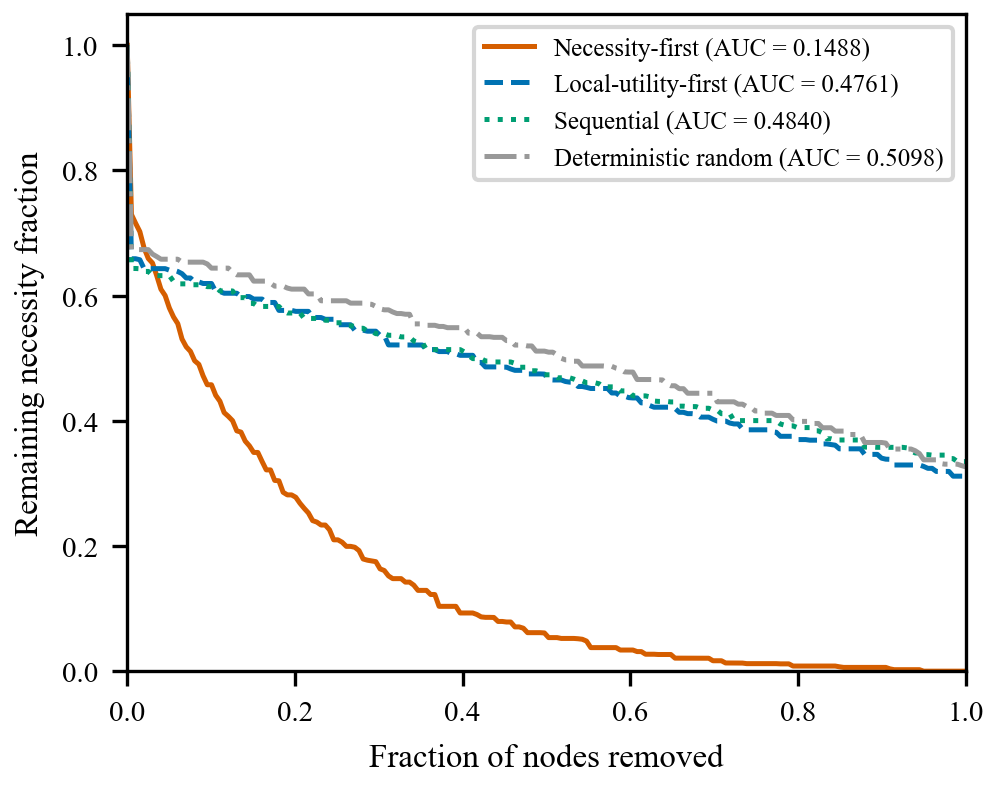
\includegraphics[width=0.88\linewidth]{figures/fig_resilience.png}
\caption{Resilience curves under ordered node removal. Four removal orders are reported: necessity-first, local-utility-first, sequential (original trace order), and deterministic random (hash-based). The $y$-axis shows remaining structural necessity fraction; the $x$-axis is the fraction of nodes removed. AUC values are annotated. The necessity-first curve degrades sharply (AUC $0.1488$), while local-utility-first (AUC $0.4761$) is close to random (AUC $0.5098$), showing that structural criticality requires graph-level diagnostics beyond local utility.}
\label{fig:resilience}
\end{figure}

Figure~\ref{fig:resilience} gives the corresponding graph-level stress view. The separation between necessity-first removal and local-utility-first removal shows that structural exposure can be hidden by local utility alone, which is why bottleneck and dependency fields are retained in the audit record.

\subsection{Role of Structural Components}

The structural components do not improve the strongest PRM800K annotation-order field in the current evidence package. Their role is narrower: when a fidelity field is strong, they expose local support, structural exposure, redundancy, and bottleneck interpretations as audit-record fields. The PRM800K route is therefore read as a strong-fidelity setting where Ridge is the conservative reportable view. The full QP objective is evaluated as the mechanism-bearing structural-allocation view, and its support comes from structural stress tests and diagnostic cases rather than from improved PRM800K annotation-order consistency.

\subsection{Hyperparameter Selection Protocol}
\label{sec:hyperparameter-selection}

The SCU weights $\alpha$, $\beta$, $\gamma$, and $\delta$ were selected before test-set reporting and then held fixed within each configuration. Development evidence from controlled synthetic calibration and development-split diagnostics set the trade-off between fidelity preservation, structural alignment, redundancy regularization, and bottleneck visibility. Locked PRM800K, audit-target retrieval, and Countries-KG test information were not used to choose these weights.

The parameters are representation controls. $\alpha$ controls fidelity preservation, $\beta$ graph-necessity alignment, $\gamma$ redundancy regularization, and $\delta$ bottleneck visibility. Reported variants keep these choices fixed to expose representation behavior.

The gamma/delta and alpha/beta QP sensitivity grids are reported as supplementary development diagnostics. They bound how the representation behaves under nearby fixed settings without treating a single grid point as external validation.

\subsection{Computational Profile}

Empirical runtime is reported separately from the asymptotic summaries. In the frozen local artifacts, the process-annotation audit-record construction run over 4,417 traces and 34,219 labeled artifacts completed in 131.57\,s on a 12-core CPU. This timing supports reproducibility; per-trace costs for the computed SC-FMA variants are reported in Supplementary Table C.7.

\begin{table}[ht]
\caption{Asymptotic time complexity for SC-FMA audit-record construction. Here $N$ is the number of artifact sequences, $k$ is the number of auditable units in a sequence, $L$ is text length, $d$ is the sparse text-feature dimension, and $I$ is the number of QP solver iterations.}
\label{tab:complexity-summary}
\centering
\small
\renewcommand{\arraystretch}{1.08}
\begin{tabular}{p{0.36\linewidth}p{0.34\linewidth}p{0.20\linewidth}}
\toprule
\textbf{Stage} & \textbf{Input size} & \textbf{Time complexity} \\
\midrule
Artifact feature extraction & $N$ sequences, $k$ units, text length $L$ & $O(NkL)$ \\
Graph construction & $k$ nodes, sparse TF-IDF features $d$ & $O(k+k^2d)$ \\
Redundancy and bottleneck diagnostics & $k$ units, similarity matrix & $O(k^2d)$ \\
Ridge calibration & $k$ artifact-feature rows & $O(k)$ after learned coefficients \\
QP calibration & $k$ units, dense constraints & $O(Ik^3)$ worst case \\
Budgeted audit-record readout & $k$ audit-record fields & $O(k\log k)$ \\
\bottomrule
\end{tabular}
\end{table}

\begin{table}[ht]
\caption{Memory profile for the same audit-record construction pipeline stages. Dense graph quantities are shown for clarity; the implementation uses sparse storage where applicable.}
\label{tab:memory-summary}
\centering
\small
\renewcommand{\arraystretch}{1.08}
\begin{tabular}{p{0.46\linewidth}p{0.38\linewidth}}
\toprule
\textbf{Stage} & \textbf{Memory complexity} \\
\midrule
Artifact feature extraction & $O(k+d)$ per sequence \\
Graph construction & $O(k^2)$ dense; sparse in implementation \\
Redundancy and bottleneck diagnostics & $O(k^2)$ \\
Ridge calibration & $O(k)$ \\
QP calibration & $O(k^2)$ \\
Budgeted audit-record readout & $O(k)$ \\
\bottomrule
\end{tabular}
\end{table}

\FloatBarrier

\section{Knowledge Engineering Representation Diagnostics}
\label{sec:application}
\label{sec:experimental-results}

This section evaluates fixed-budget audit as an information-representation task. The experiments ask whether audit records track annotation signals, whether graph construction changes dependency representations, and whether decomposed records expose audit-target information under budget constraints.

\subsection{Evaluation Philosophy: Representation Diagnostics}
\label{sec:evaluation-philosophy}

The metrics in this section are representation diagnostics. Spearman $\rho$ and Kendall $\tau$ measure whether an audit-priority field tracks the ordering of a supplied annotation or fidelity signal. NDCG, Coverage@25\%, Recall, first-selected target, and Mass@25\% measure whether relevant audit-record information remains visible under a fixed review budget. These readouts evaluate the structure and visibility of the record.

The reported values indicate fidelity tracking, coverage, or diagnostic visibility for the specified representation object under the specified data source.

\subsection{Task Definition: Fixed-Budget Knowledge Audit}
\label{sec:application-setup}

\subsubsection{Data Sources and Reference Views}

The process-annotation stage uses PRM800K phase2 records under the frozen v3.6/v3.8 hash split. A deterministic SHA-256 split over a 12,000-row source pool assigns 4,344 samples (33,555 labeled artifacts) to development and 4,417 samples (34,219 labeled artifacts) to locked reporting. The remaining 3,239 rows are retained in the split manifest but fail eligibility filters for labeled artifact coverage, split assignment, or archived feature completeness. The \wstruct{} Ridge model is fit only on development and frozen before locked reporting; the regression target is the selected PRM800K completion rating linearly mapped to $[0,1]$ as $(\mathrm{rating}+1)/2$ and clipped to the unit interval. Its feature policy forbids label fields and raw completion ratings, but the model remains supervised and uses engineered lexical, positional, numeric, and cue features. Comparisons between \wstruct{} and unsupervised structural diagnostics are therefore not equal-supervision method comparisons; the current package does not include a same-supervision structure-only Ridge control. Countries-KG tests backend feasibility. The controlled synthetic stage uses 200 traces over five fixed seeds for calibration, ablation, and error analysis. MuSiQue, WebQSP, and failed GSM8K/HotpotQA routes remain supplementary boundary diagnostics.

The frozen \wstruct{} feature list is recorded here to make the fidelity-field construction reproducible and mechanically checkable against the archived model:
% w_struct_feature_list_begin
\begin{center}
\scriptsize
\begin{tabular}{lll}
\texttt{raw\_local\_utility} & \texttt{relative\_position} & \texttt{relative\_position\_sq} \\
\texttt{relative\_position\_cu} & \texttt{log\_token\_count} & \texttt{numeric\_density} \\
\texttt{equation\_density} & \texttt{answer\_cue} & \texttt{conclusion\_cue\_count} \\
\texttt{error\_uncertainty\_cue\_count} & \texttt{reasoning\_cue\_count} & \texttt{is\_first\_step} \\
\texttt{is\_last\_step} & \texttt{trace\_step\_count} & \texttt{source\_step\_index\_ratio}
\end{tabular}
\end{center}
% w_struct_feature_list_end

Reference views include raw local utility, span length, relative position, seeded random field assignment, and stage-specific scalar views. The primary readout is annotation-order tracking for the audit-priority field, measured by Spearman $\rho$; Kendall $\tau$, record-level NDCG, and fixed-budget coverage are reported where they clarify representation visibility. Sensitivity grids, additional ablations, error modes, token-level attribution scope, and efficiency measurements are in the supplementary material.

The controlled synthetic stage tests calibration under skewed local utility, sparse necessity, and block-structured redundancy. Its annotation target combines correctness, lexical diversity, position, and structural information, which makes the audit field depend on more than one SCU input vector.

For the larger real-data stage, PRM800K is treated as a process-annotation distribution. The locked v3.6 split examines annotation-order consistency under a fixed audit budget. The v3.8 frozen PRM reference provides in-distribution prefix-sequence context. The resulting evidence concerns process-annotation audit-record behavior; deployment-oriented RAG, KG-maintenance, and human-curation workflows are discussed as future validation settings.

All reported readouts are deterministic under archived configs. The controlled synthetic stage uses five fixed seeds; confidence intervals, extended readouts, tests, and effect sizes are retained in the supplementary material.

\subsubsection{Evidence Stages and Interpretation}

The evidence is staged because each dataset tests a different part of the workflow. Table~\ref{tab:evidence-routes} states the interpretation attached to each stage.

\begin{table}[ht]
\caption{Evidence stages and interpretation. Each stage instantiates a separate part of the audit-record construction process.}
\label{tab:evidence-routes}
\centering
\small
\renewcommand{\arraystretch}{1.12}
\begin{tabular}{Z{0.27\linewidth}Z{0.27\linewidth}Z{0.34\linewidth}}
\toprule
\textbf{Evidence stage} & \textbf{Primary artifact} & \textbf{Manuscript interpretation} \\
\midrule
PRM800K process-annotation stage & 4,417 samples, 34,219 labeled artifacts & Process-annotation consistency and audit context. \\
\makecell[l]{Countries-KG backend\\feasibility study} & \makecell[l]{Fixture-level\\Countries-KG\\diagnostic} & \makecell[l]{Knowledge-graph backend\\feasibility and typed\\structural-dependency sensitivity.} \\
Audit-target retrieval stage & Rule-derived process-annotation audit targets & Lowest-overlap audit-target visibility, with aggregate context exploratory. \\
Controlled synthetic stage & 200 traces, approximately 1,000 steps, five fixed seeds & Controlled calibration and ablation evidence. \\
Frozen PRM reference & Prefix-sequence reward signals & In-distribution reference context. \\
Supplementary MuSiQue/WebQSP diagnostics & Supplementary details only & Feasibility and fixed-schema diagnostic context only. \\
Failed GSM8K/HotpotQA attempts & Failed or blocked artifacts & Transparency only; no positive evidence claim. \\
\bottomrule
\end{tabular}
\end{table}

This staged interpretation also governs null or negative results. Full QP can be too aggressive when the base fidelity field already aligns with annotation structure. The contribution is reproducible representation under stated data-generating conditions.

\subsection{Representation Fidelity Tracking on Process Annotations}
\label{sec:prm800k-evidence}

The main real-data fidelity check uses the locked PRM800K side for annotation-signal tracking and fixed-budget audit-record coverage. The stored \wstruct{} field is the primary fidelity field (Spearman $\rho = 0.611$), computed by a dev-trained frozen Ridge model. Raw local utility is negative ($\rho = -0.077$), and the overlap-limited frozen PRM prefix signal is lower ($\rho = 0.252$). SC-FMA Ridge closely tracks \wstruct{} ($\rho = 0.604$), while QP ($\rho = 0.442$) and Projection ($\rho = -0.135$) are lower-consistency variants. The archived paired-difference report does not support treating any SC-FMA variant as an annotation-order improvement over \wstruct{} on this route: Ridge differs by $-0.007$ Spearman (bootstrap CI $[-0.011,-0.004]$), QP by $-0.169$ (CI $[-0.176,-0.163]$), and Projection by $-0.746$ (CI $[-0.760,-0.732]$). This is not evidence that the redundancy and bottleneck terms improve PRM800K ranking; those terms are interpreted as structural diagnostics and conditional regularizers. Projection is the clearest failure mode: the topology-constrained simplex step can reorder artifacts when structural constraints conflict with a strong fidelity field, so it is kept as a diagnostic fallback; Ridge remains the conservative reporting variant. Supplementary Tables C.8 and C.9 report confidence intervals and fixed-budget readouts.

\begin{table}[ht]
\caption{PRM800K annotation-order consistency and fixed-budget audit coverage on the frozen split of 4,417 samples and 34,219 labeled steps. Metrics are displayed to three decimals from locked archived JSON artifacts and include all SC-FMA variants available in the locked package. N/C for the Simple average row indicates that first-selected target and Mass@25\% were not computed for this negatively correlated diagnostic reference view.}
\label{tab:prm800k-audit}
\centering
\scriptsize
\renewcommand{\arraystretch}{1.08}
\begin{tabular}{Z{0.21\linewidth}ccccZ{0.20\linewidth}}
\toprule
\textbf{Field} & \textbf{PRM $\rho$} & \textbf{First} & \textbf{Mass@25\%} & \textbf{NDCG@25\%} & \textbf{Role} \\
\midrule
\wstruct{} & \textbf{0.611} & \textbf{0.917} & \textbf{0.381} & \textbf{0.951} & Strongest real-data fidelity field. \\
SC-FMA Ridge & 0.604 & 0.905 & 0.380 & 0.946 & Close fidelity-tracking decomposition; no $\gamma/\delta$ terms. \\
SC-FMA QP & 0.442 & 0.903 & 0.379 & 0.944 & Full redundancy/bottleneck diagnostic; not the PRM800K winner. \\
SC-FMA Projection & $-$0.135 & 0.723 & 0.288 & 0.743 & Lower-consistency projection diagnostic. \\
Frozen PRM prefix signal & 0.252 & 0.777 & 0.342 & 0.847 & In-distribution reference context. \\
Raw local utility & $-$0.077 & 0.686 & 0.282 & 0.722 & Direct ablation. \\
Simple average (local utility + necessity) & $-$0.443 & N/C & N/C & 0.438 & Independent feature-average reference. \\
Random & 0.006 & 0.733 & 0.307 & 0.776 & Seeded sanity control. \\
\bottomrule
\end{tabular}
\end{table}

Table~\ref{tab:prm800k-audit} shows annotation-order behavior on a process-annotation distribution. The normalized fidelity input $\tilde{\mathbf{c}}$ is instantiated by the supervised \wstruct{} field, and Ridge closely tracks this field while adding diagnostic decomposition. The archived fixed-budget readouts show a small tracking cost (Mass@25\% 0.3809 for \wstruct{} versus 0.3796 for Ridge; Coverage NDCG@25\% 0.9506 versus 0.9460). The simple-average reference view (unweighted mean of raw local utility and structural necessity, Spearman $\rho = -0.443$) loses annotation-order consistency. Its component audit explains the sign: raw local utility is weakly negative ($\rho=-0.077$), and the structural-necessity input alone is more strongly anti-correlated with the PRM800K labels ($\rho=-0.418$). This negative direction means the current time-adjacent and TF-IDF graph construction is not merely low-yield in this domain; it is directionally misaligned with the human process labels under this readout. Thus, in this real-data route, naive averaging of raw utility with structural necessity is not trustworthy; a learned fidelity field and a conservative Ridge combination are needed when annotation fidelity is already strong. Because no same-supervision structure-only Ridge control is reported, the comparison cannot establish that a supervised structural model would fail under equal training signal.

\subsection{Representation Enrichment Analysis}
\label{sec:representation-enrichment}

The close correlation between \wstruct{} and SC-FMA Ridge makes the enrichment analysis central. We compare three views already stored or derivable in the locked audit-card auto-validation artifact: a scalar \wstruct{} representation, a raw-field bundle that exposes fidelity, raw local utility, structural necessity, redundancy density, and bottleneck indicators without SCU joint optimization, and the structured SC-FMA view with recommended actions and utility-anchor interpretation fields.

\textbf{Field enrichment.} The scalar baseline exposes one field: \texttt{w\_struct\_scalar}. The raw-field bundle exposes five unoptimized fields: fidelity, raw local utility, structural necessity, redundancy density, and bottleneck indicator. The SC-FMA view exposes six fields: fidelity, structural necessity, redundancy, bottleneck status, recommended action, and upstream utility-anchor status. These fields operationalize dependency, redundancy, bottleneck, structural-role, diagnostic-reason, and utility-anchor dimensions. The raw-field bundle is included to test whether the retrieval gain comes merely from exposing more fields.

\begin{table}[ht]
\caption{Representation enrichment relative to a scalar \wstruct{} field. Counts are taken from the locked audit-card auto-validation artifact and report additional audit-record fields and diagnostic categories.}
\label{tab:representation-enrichment}
\centering
\scriptsize
\renewcommand{\arraystretch}{1.08}
\begin{tabular}{Z{0.24\linewidth}cccccc r}
\toprule
\textbf{Representation} & \textbf{Fid.} & \textbf{Dep.} & \textbf{Red.} & \textbf{Bot.} & \textbf{Reason} & \textbf{Anchor} & \textbf{Fields} \\
\midrule
\wstruct{} scalar & \checkmark & -- & -- & -- & -- & -- & 1 \\
Raw field bundle & \checkmark & \checkmark & \checkmark & \checkmark & -- & \checkmark & 5 \\
SC-FMA record & \checkmark & \checkmark & \checkmark & \checkmark & \checkmark & \checkmark & 6 \\
\bottomrule
\end{tabular}
\end{table}

The same artifact records four unique diagnostic target categories: weak utility anchor, structural over-correction, redundancy consolidation, and bottleneck protection. Under the fixed 25\% inspection budget, the raw-field bundle raises mean rule-target recall from 0.235 to 0.524 and mean NDCG from 0.353 to 0.768, showing that field exposure explains a large share of the automatic retrieval signal. The SC-FMA view further raises mean recall to 0.699 and mean NDCG to 0.978. The largest numerical delta occurs on bottleneck protection, but that target is defined from QP top-25\% budget entry and is therefore read as an internal record-consistency check rather than independent audit-target retrieval. Following the interpretation rule in Section~\ref{sec:evaluation-philosophy}, these values are diagnostic-separation readouts; the main lowest-overlap subset is analyzed separately in Section~\ref{sec:why-calibration}.

\begin{table}[ht]
\caption{Diagnostic-category separation under the fixed 25\% audit budget. The targets are rule-derived categories in the locked audit-card auto-validation artifact. The bottleneck-protection row is QP-derived and should be read as internal record consistency.}
\label{tab:diagnostic-separation}
\centering
\small
\renewcommand{\arraystretch}{1.08}
\begin{tabular}{Z{0.27\linewidth}rrrr}
\toprule
\textbf{Diagnostic category} & \textbf{Positive cases} & \textbf{\wstruct{} recall} & \textbf{Raw-field recall} & \textbf{SC-FMA recall} \\
\midrule
Weak utility anchor & 2,420 & 0.247 & 0.455 & 0.455 \\
Structural over-correction & 2,145 & 0.228 & 0.430 & 0.515 \\
Redundancy consolidation & 1,214 & 0.199 & 0.762 & 0.824 \\
Bottleneck protection & 382 & 0.264 & 0.450 & 1.000 \\
\bottomrule
\end{tabular}
\end{table}

\textbf{Representation disagreement cases.} At the locked-summary level, Ridge is close to \wstruct{} on annotation-order consistency (0.604 versus 0.611), while QP is more distinct (0.442). Ridge is intentionally fidelity-tracking-oriented. QP shows how the summary order changes when the record shifts from fidelity tracking toward constrained structural allocation. The archived package stores summary readouts for these variants; per-artifact top-$k$ overlap and rank-change ratios are outside the stored artifact schema.

\textbf{Diagnostic separation.} The clearest enrichment appears when artifacts or traces have similar scalar-fidelity visibility but different audit reasons. Under the same 25\% budget, raw fields already separate many weak utility-anchor and redundancy cases that the scalar view collapses. SC-FMA adds beyond raw fields where a record-level interpretation is needed, especially structural over-correction and redundancy consolidation. The bottleneck-protection row checks whether the SC-FMA record exposes a QP-derived protected-bottleneck state; it is not independent retrieval evidence. These readouts support the representation-level claim that SC-FMA increases diagnostic organization, not the stronger claim that SCU optimization alone explains all retrieval gains.

\subsection{Knowledge-Graph Backend Feasibility Study}
\label{sec:kg-pilot}

The Countries-KG backend feasibility study examines typed graph ingestion within the audit-record interface. As a diagnostic check on non-lexical graph construction, we use the Countries KG resource associated with approximate-reasoning evaluation over country, region, and neighborhood relations~\cite{bouchard2015approximate}. The fixture contains 30 entities and 189 triples over \texttt{locatedIn} and \texttt{neighborOf}. We generate 30 deterministic KG-query traces and construct both a lightweight lexical-dependency graph and a KG-augmented graph that maps ontology relations to functional edge types.

\begin{table}[ht]
\caption{Countries-KG backend feasibility study (30 traces over a real knowledge graph, 30 entities, 189 triples). KG-augmented edges are derived from typed ontology relations. Structural-necessity consistency is the archived rank-consistency diagnostic between TF-IDF reference and KG-augmented necessity fields; the reported 0.0 is the rounded archived value under that computation.}
\label{tab:kg-pilot}
\centering
\small
\renewcommand{\arraystretch}{1.08}
\begin{tabular}{Z{0.45\linewidth}Z{0.43\linewidth}}
\toprule
\textbf{Quantity} & \textbf{Value} \\
\midrule
KG entities / triples & 30 / 189 \\
KG relation types & \texttt{locatedIn}, \texttt{neighborOf} \\
Reasoning traces & 30 \\
TF-IDF reference edges & 310 \\
KG candidate edges & 304 \\
KG-augmented edges & 320 \\
KG-derived edges added & 196 \\
Ontology relations detected & depends\_on\_concept (211), same\_constraint (85), neighbor\_concept (8) \\
Mean abs structural-necessity delta & 0.431 \\
Structural-necessity consistency (reference vs KG) & 0.0 \\
Bottleneck top-1 overlap & 1.000 \\
Matched nodes & 154 \\
\bottomrule
\end{tabular}
\end{table}

Table~\ref{tab:kg-pilot} shows that typed KG edges change the graph substantially: the stage considers 304 KG candidate relations, adds 196 ontology-derived edges, and yields 320 KG-augmented graph edges versus 310 TF-IDF reference edges. The mean absolute structural-necessity delta is 0.431 with an archived reference-vs-KG necessity consistency rounded to 0.0. One reading is that KG augmentation changes which objects the representation marks as structurally dependent. The equally important caution is that the structural-necessity field is highly sensitive to the graph-construction backend in this fixture; this sensitivity is a reliability warning, not a validation win. The 30-trace fixture is proof-of-concept evidence for typed backend substitution and a methodological analogy to knowledge-graph curation: the evidence concerns the graph-construction interface, not production-scale ontology validation or a live knowledge-base audit workflow. Full edge lists, the diagnostic report, and degeneracy-handling details are in the supplementary material.
% Scope note for tests: fixture-level typed-edge construction only; no deployed workflow validation.

\subsection{Rule-Derived Audit Record Retrieval Diagnostic}
\label{sec:why-calibration}
\label{sec:audit-results}
\label{sec:oracle-auto-validation}

The audit-target retrieval stage examines whether decomposition fields make rule-derived audit targets visible under a fixed review budget. The main readout is the weak utility-anchor family, which has the lowest direct overlap with the exposed SC-FMA output fields. In this stage, \wstruct{} is the frozen scalar fidelity signal supplied to the record builder. The weak utility-anchor rule uses this input-side fidelity repair pattern; redundancy and structural-over-correction targets reuse fields that SC-FMA exposes, and bottleneck protection directly reuses QP budget entry. The raw-field bundle is therefore reported alongside SC-FMA to separate field exposure from SCU joint optimization.

We evaluate failure-mode localization as retrieval over traces. The scalar-only view receives the \wstruct{} summary, the raw-field view receives unoptimized primitive fields, and the SC-FMA view receives fidelity, necessity, redundancy, bottleneck status, recommended-action, and interpretation fields. Automatic oracle targets come from frozen process-annotation labels, priority-field disagreements, redundancy density, bottleneck flags, and the failure-taxonomy rules in Appendix~\ref{app:failure-taxonomy}. Weak utility-anchor targets have the lowest direct field overlap; redundancy consolidation and structural over-correction provide partially overlapping diagnostic context. Bottleneck protection is QP-derived by construction and is treated separately as a record-consistency check.

The target-family rules are fixed before scoring and are implemented as explicit threshold tests. In compact form: structural over-correction is assigned when $\rho_{\mathrm{QP}}\le \rho_{\wstruct{}}-0.10$; redundancy consolidation when redundancy density is in the top tertile and QP trails $\max(\rho_{\mathrm{Ridge}},\rho_{\wstruct{}})$ by at least 0.05; bottleneck protection when a bottleneck step enters the QP top-25\% budget while its process label is below the trace median; and weak utility anchor when $\rho_{\mathrm{raw}}\le 0$ and $\rho_{\wstruct{}}\ge 0.30$. These labels are multi-label and not mutually exclusive. Because the bottleneck-protection definition directly uses QP budget entry, its SC-FMA score checks whether the audit record reflects an internally computed QP bottleneck state. It is not an independent target-retrieval validation. Weak utility-anchor is the lowest direct-overlap rule, but it is still not fully independent because it uses \wstruct{} as an input-side fidelity signal.

\begin{table}[ht]
\caption{Field-overlap audit for rule-derived target families. Overlap is the number of SC-FMA decomposition fields directly reused by the target rule divided by the six fields exposed in the archived SC-FMA view.}
\label{tab:target-circularity-audit}
\centering
\scriptsize
\renewcommand{\arraystretch}{1.08}
\begin{tabular}{Z{0.21\linewidth}Z{0.25\linewidth}cZ{0.22\linewidth}Z{0.14\linewidth}}
\toprule
\textbf{Target family} & \textbf{Fields used by target rule} & \textbf{Overlap} & \textbf{SC-FMA field relation} & \textbf{Interpretation} \\
\midrule
Weak utility anchor & Process labels, raw local utility, frozen \wstruct{} fidelity-field repair pattern & 1/6 & Lowest direct overlap; uses an input-side fidelity repair pattern & Main low-overlap retrieval check \\
Redundancy consolidation & Redundancy density, redundant-cluster flags, priority change & 2/6 & Partial overlap through redundancy and recommended-action fields & Exploratory diagnostic \\
Bottleneck protection & Bottleneck flag, QP top-25\% budget entry, below-median process label & 2/6 & QP-derived through bottleneck and budget-entry fields & Internal consistency check \\
Structural over-correction & Fidelity-vs-structure disagreement, QP/Ridge priority divergence & 2/6 & Partial overlap through fidelity and necessity disagreement fields & Exploratory diagnostic \\
\bottomrule
\end{tabular}
\end{table}

\begin{table}[ht]
\caption{Per-target audit-target retrieval point estimates under the same 25\% budget. Field overlap reports the approximate definition overlap with the six SC-FMA decomposition fields. The weak utility-anchor row is the main lowest-overlap check, but it still uses the input-side \wstruct{} fidelity pattern; asterisks mark target families with stronger definitional overlap. The bottleneck-protection row is QP-derived and is reported as an internal consistency check.}
\label{tab:oracle-auto-validation-by-target}
\centering
\scriptsize
\renewcommand{\arraystretch}{1.08}
\begin{tabular}{Z{0.21\linewidth}rZ{0.09\linewidth}cccccc}
\toprule
\textbf{Target family} & \textbf{Pos.} & \textbf{Overlap} & \textbf{\wstruct{} R} & \textbf{Raw R} & \textbf{SC-FMA R} & \textbf{\wstruct{} N} & \textbf{Raw N} & \textbf{SC-FMA N} \\
\midrule
Bottleneck protection\textsuperscript{*} & 382 & 2/6 QP & 0.264 & 0.450 & 1.000 & 0.221 & 0.411 & 1.000 \\
Redundancy consolidation\textsuperscript{*} & 1,214 & 2/6 & 0.199 & 0.762 & 0.824 & 0.224 & 0.849 & 0.916 \\
Weak utility anchor & 2,420 & 1/6 input & 0.247 & 0.455 & 0.455 & 0.527 & 0.997 & 0.997 \\
Structural over-correction\textsuperscript{*} & 2,145 & 2/6 & 0.228 & 0.430 & 0.515 & 0.439 & 0.817 & 1.000 \\
\bottomrule
\end{tabular}
\end{table}

The weak utility-anchor row provides the lowest-direct-overlap subset check in the locked artifact and is the main audit-target retrieval readout. The raw-field and SC-FMA rows are identical on this target, so this subset does not show an SCU-specific retrieval advantage. The rule uses process labels and the frozen \wstruct{} fidelity signal from the same archived package. The input-output distinction is important: \wstruct{} supplies the scalar fidelity field for this stage, raw fields expose primitive components, and the SC-FMA output adds record-level dependency, redundancy, bottleneck, reason, and interpretation fields. The per-target rows are point estimates; the archived aggregate report stores bootstrap intervals only for the aggregate retrieval table below. Table~\ref{tab:oracle-auto-validation} reports aggregate automatic retrieval as contextual evidence because targets with definitional overlap account for 3,741 of 6,161 target positions (about 61\%).

\begin{table}[ht]
\caption{Aggregate retrieval under partially overlapping target definitions. Failure-mode localization is evaluated on the locked PRM800K split as a representation-coverage diagnostic under a 25\% budget. The scalar condition uses \wstruct{}, the raw-field bundle exposes primitive fields without SCU joint optimization, and the SC-FMA condition uses decomposition and interpretation fields. The main low-overlap retrieval check is the weak utility-anchor row in Table~\ref{tab:oracle-auto-validation-by-target}; bottleneck protection is QP-derived internal consistency.}
\label{tab:oracle-auto-validation}
\centering
\scriptsize
\renewcommand{\arraystretch}{1.08}
\begin{tabular}{Z{0.30\linewidth}ccccc}
\toprule
\textbf{View} & \textbf{Cov.@25\%} & \textbf{NDCG@25\%} & \textbf{MRR} & \textbf{First} & \textbf{Cost} \\
\midrule
\wstruct{} scalar only & 0.235 & 0.353 & 0.354 & 0.000 & 0.0007 \\
Raw field bundle & 0.524 & 0.768 & 1.000 & 1.000 & 0.0002 \\
SC-FMA decomposition & 0.699 & 0.978 & 1.000 & 1.000 & 0.0002 \\
\bottomrule
\end{tabular}
\end{table}

The aggregate difference is exploratory recovery of rule-defined audit targets by a decomposed audit record. The archived aggregate bootstrap intervals are wide for coverage and NDCG: \wstruct{} coverage $[0.211,0.256]$ and NDCG $[0.222,0.483]$, raw-field coverage $[0.435,0.684]$ and NDCG $[0.521,0.952]$, and SC-FMA coverage $[0.485,0.912]$ and NDCG $[0.937,1.000]$. These intervals do not remove the definitional-overlap concern. The diagnostic checks whether the record fields are machine-readable; independent audit quality remains a human-validation question. The raw-field control shows that much of the gain comes from exposing primitive fields, while SC-FMA adds record-level organization and additional retrieval mainly for redundancy and structural-overcorrection families. The bottleneck contribution is interpreted as QP-derived internal consistency rather than independent evidence. Table~\ref{tab:compact-audit-card-case} gives one compact preview case; the appendix Audit Cards provide fuller trace-level examples.

\begin{table}[H]
\caption{Compact Audit Card case study: scalar-only view versus SC-FMA decomposition.}
\label{tab:compact-audit-card-case}
\centering
\small
\renewcommand{\arraystretch}{1.08}
\begin{tabular}{Z{0.22\linewidth}Z{0.30\linewidth}Z{0.36\linewidth}}
\toprule
\textbf{Failure target} & \textbf{\texttt{wstruct}-only view} & \textbf{SC-FMA Audit Card view} \\
\midrule
Bottleneck protection & A scalar signal can allocate a step for early inspection while leaving downstream gating implicit. & Bottleneck and necessity fields mark the step as dependency-exposed, so the interpretation is to inspect the downstream chain before dropping it. \\
Redundancy consolidation & Multiple high-signal steps can look independently important. & Redundancy density and neighborhood fields identify a cluster, so the interpretation is to consolidate the checks or sample the cluster. \\
Weak utility anchor & A high calibrated fidelity field can hide a failed raw local utility signal. & Fidelity and raw-anchor disagreement expose an upstream utility-anchor problem, so the interpretation is to diagnose the signal source. \\
\bottomrule
\end{tabular}
\end{table}

\subsection{Controlled Calibration Analysis}
\label{sec:controlled-calibration}

\begin{table}[ht]
\caption{Controlled representation-field assignment on the synthetic stage. For SC-FMA variants, Spearman $\rho$ is the 5-seed mean $\pm$ standard deviation; remaining columns are from representative seed 42 because the archived multiseed run records Spearman alone. Simple average is the element-wise mean of normalized local utility and structural necessity.}
\label{tab:controlled-calibration-results}
\centering
\small
\begin{tabular}{Z{0.30\linewidth}cccc}
\toprule
\textbf{View} & \textbf{Synthetic label $\rho$} & \textbf{Kendall $\tau$} & \textbf{Record NDCG@3} & \textbf{Record NDCG@5} \\
\midrule
SC-FMA QP                  & \textbf{0.597} $\pm$ 0.064 & 0.533 & 0.921 & 0.958 \\
SC-FMA Ridge               & 0.541 $\pm$ 0.016 & 0.447 & 0.889 & 0.927 \\
Raw local utility          & 0.483 & 0.412 & 0.874 & 0.919 \\
Simple average (local utility + necessity) & 0.478 & 0.413 & 0.889 & 0.926 \\
SC-FMA Projection          & 0.372 $\pm$ 0.030 & 0.278 & 0.824 & 0.890 \\
Span Length                & $-$0.006 & $-$0.013 & 0.740 & 0.826 \\
Relative Position          & $-$0.005 & $-$0.004 & 0.735 & 0.827 \\
Random                     & $-$0.010 & $-$0.008 & 0.736 & 0.825 \\
\bottomrule
\end{tabular}
\end{table}

Table~\ref{tab:controlled-calibration-results} shows the intended calibration behavior: SC-FMA QP records higher annotation-order consistency than raw local utility, with a Spearman gap of 0.114. Under the controlled annotation target, structural calibration improves local-utility field assignment.

\begin{table}[ht]
\caption{SCU component contribution on the controlled synthetic stage. Values are 5-seed mean $\pm$ standard deviation over seeds 42, 123, 456, 789, and 1024. Delta is the annotation-order consistency difference relative to \texttt{full\_scu}. The largest drop occurs when the fidelity signal is removed; removing redundancy or bottleneck regularization has near-zero impact on the reported consistency readouts in this setting.}
\label{tab:scu-component-contribution}
\centering
\small
\renewcommand{\arraystretch}{1.08}
\begin{tabular}{lccc}
\toprule
\textbf{Variant} & \textbf{Synthetic label $\rho$ mean$\pm$std} & \textbf{Kendall $\tau$ mean$\pm$std} & \textbf{Delta vs Full} \\
\midrule
\texttt{full\_scu} & 0.5103 $\pm$ 0.0320 & 0.4297 $\pm$ 0.0287 & 0.0000 \\
\texttt{no\_fidelity} & 0.2850 $\pm$ 0.0153 & 0.2366 $\pm$ 0.0138 & $-$0.2253 \\
\texttt{no\_structure} & 0.4841 $\pm$ 0.0334 & 0.4053 $\pm$ 0.0285 & $-$0.0263 \\
\texttt{no\_redundancy} & 0.5093 $\pm$ 0.0321 & 0.4273 $\pm$ 0.0273 & $-$0.0010 \\
\texttt{no\_bottleneck} & 0.5090 $\pm$ 0.0304 & 0.4279 $\pm$ 0.0274 & $-$0.0013 \\
\bottomrule
\end{tabular}
\end{table}

Table~\ref{tab:scu-component-contribution} refines the component narrative. Removing fidelity reduces annotation consistency by 0.2253, far more than any other removal. Graph necessity contributes moderately (Delta $=-0.0263$), while redundancy and bottleneck change consistency by about 0.001. Here, those terms mainly provide regularization and decomposition. For annotation-order consistency alone, the simplified Ridge view is often sufficient; redundancy and bottleneck fields matter most when the audit task asks why a selected artifact is duplicated, dependency-exposed, or protected under a fixed budget.

The near-zero redundancy and bottleneck deltas reflect the structure-independent proxy label. We therefore use a structural stress-test (Table~\ref{tab:scu-stress-test}) whose labels encode redundancy-awareness and bottleneck protection.

\begin{table}[ht]
\caption{SCU component contribution on a structural stress-test fixture (200 traces per seed, five fixed seeds 42, 123, 456, 789, 1024). These designed labels reward redundancy-awareness and bottleneck protection under a stress-test redundancy setting ($\gamma=0.6$). Delta is the annotation-order consistency difference relative to \texttt{full\_scu}. The table is an implementation and mechanism diagnostic, not real-data audit-value evidence.}
\label{tab:scu-stress-test}
\centering
\small
\renewcommand{\arraystretch}{1.08}
\begin{tabular}{lccc}
\toprule
\textbf{Variant} & \textbf{Stress-label $\rho$ mean$\pm$std} & \textbf{Kendall $\tau$ mean$\pm$std} & \textbf{Delta vs Full} \\
\midrule
\texttt{full\_scu} & 0.6249 $\pm$ 0.0145 & 0.5238 $\pm$ 0.0112 & 0.0000 \\
\texttt{no\_fidelity} & 0.4832 $\pm$ 0.0357 & 0.3935 $\pm$ 0.0319 & $-$0.1417 \\
\texttt{no\_structure} & 0.5871 $\pm$ 0.0234 & 0.4870 $\pm$ 0.0224 & $-$0.0378 \\
\texttt{no\_redundancy} & 0.5758 $\pm$ 0.0163 & 0.4889 $\pm$ 0.0091 & $-$0.0492 \\
\texttt{no\_bottleneck} & 0.5409 $\pm$ 0.0145 & 0.4424 $\pm$ 0.0114 & $-$0.0840 \\
\bottomrule
\end{tabular}
\end{table}

On the stress-test, removing fidelity costs the most ($-0.1417$). Structural terms also contribute: bottleneck log-barrier $0.0840$, redundancy penalty $0.0492$, and structural-dependency term $0.0378$. Redundancy and bottleneck act as conditional regularizers whose contribution grows when the fidelity signal lacks structural preference or when high-redundancy blocks make audit interpretation depend on cluster structure.

\begin{table}[ht]
\caption{Graph construction analysis on the diagnostic run. Temporal edges define the primary backbone; topical similarity edges are supplementary cues. Record NDCG@3 and Record NDCG@5 are interpreted as budget-constrained audit-coverage readouts computed from the same diagnostic-run source data and metric definition used for the correlation readout.}
\label{tab:graph-construction-analysis}
\centering
\small
\renewcommand{\arraystretch}{1.08}
\begin{tabular}{lcccc}
\toprule
\textbf{Variant} & \textbf{Graph diagnostic $\rho$} & \textbf{Kendall $\tau$} & \textbf{Record NDCG@3} & \textbf{Record NDCG@5} \\
\midrule
\texttt{full\_tfidf} & 0.0515 & 0.0458 & 0.8655 & 0.8655 \\
\texttt{temporal\_only} & 0.0596 & 0.0527 & 0.8688 & 0.8688 \\
\texttt{jaccard\_topical} & 0.0517 & 0.0460 & 0.8657 & 0.8657 \\
\texttt{shuffled\_topical} & 0.0515 & 0.0458 & 0.8655 & 0.8655 \\
\bottomrule
\end{tabular}
\end{table}

Table~\ref{tab:graph-construction-analysis} shows that topical edges add little annotation-signal tracking evidence: \texttt{full\_tfidf} is slightly below \texttt{temporal\_only} and matches \texttt{shuffled\_topical}. Their observed role is supplementary structural cueing.

The reference-view pattern clarifies the source of the representation signal. Raw local utility carries more annotation-order information than span length, position, and random controls but is still negative on the locked process-annotation route. Plain averaging of local utility and structural necessity is worse than either conservative \wstruct{} or Ridge because the structural-necessity input is not independently aligned with PRM800K labels in that setting. The archived workflow is defined at the artifact-step level.

The component and graph-construction analyses clarify how the representation is built. SCU benefits primarily from fidelity-signal tracking and only conditionally from graph-necessity alignment. On the PRM800K route, graph necessity is directionally misaligned with human labels; on the designed stress-test, structural terms help because the labels encode the structural preference by construction. Redundancy and bottleneck terms mainly support conservative decomposition. Topical graph edges move structural diagnostics while leaving annotation-order consistency largely unchanged.

Error analysis identifies three residual patterns: high-utility but zero-necessity steps can receive excessive mass; near-threshold bottlenecks can be under-protected; and dense redundancy blocks can over-equalize priority values.

\subsection{Failure Modes of Representation Layer}
\label{sec:prm800k-error}

The stratified audit-record diagnostics show when structural calibration helps or hinders process-annotation consistency. The multi-label failure taxonomy over 4,417 locked traces reports weak utility anchor in 54.79\% of traces, structural over-correction in 48.56\%, redundancy misclassification in 27.48\%, low signal or tie in 18.32\%, and bottleneck over-protection in 8.65\%. Fixed-template Audit Cards are provided in Appendix~\ref{app:failure-taxonomy}.

Trace length is an important observed predictor of variant behavior and a practical limitation for the full QP variant. On short traces (7,141 steps across 1,806 samples), \wstruct{} reaches Spearman $\rho = 0.759$, Ridge closely tracks it at 0.757, and QP remains close at 0.734. The middle trace-length stratum (8,264 steps across 1,195 samples) is intermediate: \wstruct{} is 0.583, Ridge is 0.579, and QP is 0.321. On long traces (18,814 steps, 1,416 samples), \wstruct{} drops to 0.447, Ridge to 0.430, and QP degrades to 0.172. Longer and more complex traces are exactly where audit support is often needed, so this degradation is operationally important rather than a minor tail case. Longer traces likely create denser redundancy blocks; QP's hard penalty then reallocates the audit-priority field away from the annotation signal, while Ridge's soft averaging avoids the sharpest overcorrection. This pattern motivates a future engineering extension: sparse, blockwise, or windowed calibration could reduce the effective $k$ in the constrained subproblem while preserving the same SCU record fields.

Label entropy gives a complementary view. On low-entropy traces (17,288 steps, 1,474 samples), discriminability is limited but \wstruct{} and Ridge still record Coverage NDCG@25\% above 0.99 as a fixed-budget audit-coverage readout. The middle entropy stratum (10,948 steps across 1,639 samples) gives \wstruct{} 0.642, Ridge 0.632, and QP 0.501. On high-entropy traces (5,983 steps, 1,304 samples), labels are more dispersed and QP ($\rho = 0.642$) moves closer to \wstruct{} ($\rho = 0.705$), suggesting that explicit redundancy management is more useful when annotation structure is richer.

Across strata, \wstruct{} provides the main fidelity reference, Ridge stays within 0.01--0.02 Spearman $\rho$ across most strata, QP degrades on long or high-redundancy traces, and Projection provides the least consistent SC-FMA representation variant. The frozen PRM prefix signal provides moderate in-distribution reference context (Spearman 0.061--0.425) and remains consistently above raw local utility.

\section{Discussion}
\label{sec:discussion}

\subsection{Graph-Aware Calibration in the Knowledge Lifecycle}
\label{sec:knowledge-lifecycle}

Knowledge-intensive systems expose artifacts during construction, retrieval, validation, update, and reuse. These artifacts vary in structural role and diagnostic implication. Earlier knowledge-engineering and curation work emphasized inspectable intermediate states and maintenance-oriented review~\cite{buchanan1984mycin,laird2012soar,studer1998knowledge,higgins2008dcc}. Recent KG prompting, engineering-design RAG, KG-quality, and algorithm-auditing studies show why inspection remains difficult when structured knowledge is noisy, incomplete, redundant, or stale~\cite{dai2025llmkg,siddharth2024retrieval,chen2025kgquality,dwivedi2021artificial,raji2020closing}.

For knowledge curation, the useful object is the record that travels with an artifact after scoring. It states why the artifact was selected, which neighboring artifacts it depends on, and whether the selected evidence is duplicated or dependency-exposed.

The empirical evidence makes this interpretation concrete, but also narrows it. Ridge remains close to the supplied PRM800K fidelity field, while the enrichment and retrieval diagnostics show that similar priority values can require different maintenance actions. The graph-construction ablation and the negative structural-necessity correlation temper the role of the default TF-IDF topology: in the current evidence package, it behaves as a replaceable and fragile graph interface rather than as an independently aligned mathematical-reasoning dependency model.

The contribution is a reusable audit-record schema for knowledge-representation workflows. It gives curators a stable representation object for inspecting, comparing, and reusing process artifacts under a fixed review budget.

\subsection{Audit Records for Maintenance-Oriented Analysis}
\label{sec:audit-interpretation}

During maintenance, the audit record links a selected artifact to a practical reading: verify the fidelity signal, inspect a dependency chain, consolidate duplicate evidence, or protect a bottleneck.

The process-annotation stratification shows how these readings appear in archived traces. Weak utility-anchor cases indicate when the fidelity signal should be repaired; structural-over-correction cases mark excessive graph regularization; redundancy cases identify clusters; and bottleneck cases identify dependency-exposed objects.

Budget-constrained audit coverage, first-selected target, and Mass@25\% match this fixed-budget setting more directly than whole-trace correlation alone. Local evidence signals such as retrieval confidence, entity-linking similarity, and rule-certainty factors can duplicate earlier checks or miss dependency-exposed objects; SC-FMA records those distinctions.

The variant evidence suggests a practical policy. When fidelity is strong, Ridge keeps the record close to the supplied signal; when fidelity and structure diverge, QP-style diagnostics are worth checking during development.

\subsection{Variant-Selection Guidance}

Table~\ref{tab:variant-policy} converts the stratified diagnosis into observed development patterns, not a prospectively validated selector. The thresholds are calibrated to the present development evidence. The $\rho \ge 0.50$ and $\rho < 0.30$ cut points come from the development-set pattern in which Ridge stays within about 0.02 Spearman of a strong fidelity field, while QP becomes worth checking when structural-term ablations or sensitivity grids change development Spearman by about 0.03 or more. The supporting QP grids are reported in the supplementary hyperparameter tables. Ridge is the conservative default when ground-truth audit labels are unavailable because it tracks a strong fidelity field while exposing diagnostic fields. QP is appropriate when development diagnostics or domain knowledge indicate that scalar fidelity is structurally blind, but the PRM800K long-trace stratum shows that QP can be brittle when dense redundancy competes with the fidelity signal. Projection is retained as a fast diagnostic.

Ridge is the development choice when a fidelity signal already aligns with annotations, as in the locked process-annotation stage. QP should be evaluated when utility and structure are expected to disagree and redundancy management is central. Projection is computationally simple but brittle when structural signal conflicts with the fidelity signal. A ground-truth-free selector based on fidelity-structure divergence, rank instability, and ensemble agreement is left to future work.

\begin{table}[ht]
\caption{Observed Ridge/QP development patterns derived from the stratified analysis. Thresholds are post-hoc development-set heuristics from the present evidence package, not a prospectively validated selection rule.}
\label{tab:variant-policy}
\centering
\small
\renewcommand{\arraystretch}{1.08}
\begin{tabular}{Z{0.32\linewidth}Z{0.42\linewidth}Z{0.16\linewidth}}
\toprule
\textbf{Setting} & \textbf{Development diagnostic} & \textbf{Recommendation} \\
\midrule
Well-aligned fidelity field, as in process-annotation distributions & Fidelity-field annotation-order consistency is high on development data (roughly $\rho \ge 0.50$ here), and Ridge remains within about 0.02 Spearman of that field. & Ridge \\
Weak or structurally blind fidelity field & Fidelity consistency is low (roughly $\rho < 0.30$), simple feature averaging fails, or stress-test/component ablations show structural-term removals changing development Spearman by at least 0.03. & Evaluate QP first \\
Unclear structure or runtime-critical setting & Structural diagnostics are immature, or iterative QP calibration exceeds the available runtime budget. & Ridge; Projection as diagnostic fallback \\
\bottomrule
\end{tabular}
\end{table}

\subsection{Scope and Limitations}
\label{sec:scope-limitations}

\medskip
\noindent The current evidence supports audit-record construction and representation-level knowledge-engineering claims. Deployment-oriented knowledge-base maintenance and human audit-use protocols remain future validation settings.
% Scope note for tests: audit-record representation evidence only; no deployed workflow validation.

\medskip
\noindent\textbf{Data and signal boundaries.} The synthetic calibration stage is controlled and proxy-labeled, while the locked process-annotation stage supports annotation-order consistency and fixed-budget audit within a PRM800K-derived annotation distribution. SC-FMA Ridge is reported as fidelity-tracking decomposition relative to \wstruct{}, not as an improvement over \wstruct{} on this route. The strongest baseline is a supervised Ridge fidelity field with engineered lexical, positional, numeric, and cue features; the current evidence package does not include a same-supervision structure-only Ridge baseline, so the structural terms should not be interpreted as having lost a fair supervised baseline comparison. Mathematical step annotations are used as process-annotation artifacts. The binary-correctness local utility signal is a coarse trace-level utility anchor, and the resulting audit-priority field values are local representation signals. Causal effect estimates would require a separate identification design.

\textbf{Graph-construction boundary.} The fallback lexical graph uses temporal order and TF-IDF topical similarity. The Sentence-BERT ablation and Countries-KG typed-edge stage show backend substitutability under diagnostic conditions. TF-IDF topical edges did not improve annotation-order tracking over temporal-only edges in the archived ablation, and structural necessity is anti-correlated with PRM800K labels under the current construction. The Countries-KG result is a methodological analogy and graph-interface diagnostic based on 30 traces, not production knowledge-graph validation; its 0.0 reference-vs-KG consistency also shows backend sensitivity. Stronger topology construction and domain-specific dependency graphs remain open directions.

\textbf{Audit-retrieval boundary.} The audit-target retrieval evidence is rule-derived. The weak utility-anchor subset is the main lowest-direct-overlap retrieval evidence, while the aggregate result summarizes target families with definitional overlap. The bottleneck-protection family is defined through QP top-budget entry and is therefore an internal record-consistency check, not independent retrieval evidence. The weak utility-anchor rule uses \wstruct{} as an input-side fidelity signal, and the raw-field bundle matches SC-FMA on this target. The target-family rules support reproducibility; automatic retrieval diagnostics establish record visibility, while human audit usefulness requires expert adjudication.

\textbf{Operational boundary.} QP is the most complete SCU variant but degrades sharply on long PRM800K traces. This limits the current full-objective implementation for the settings where audit support may be most valuable. Human-in-the-loop comparison between scalar views, raw-field bundles, and SC-FMA audit records is required before making claims about reviewer speed, curator accuracy, actionability, or maintenance usefulness.

\medskip
\noindent\textbf{Scope exclusions.} Downstream PRM training, production knowledge-base deployment, causal identification, and external PRM generalization are outside the current evidence boundary.

\noindent Within these bounds, SC-FMA points to a knowledge-lifecycle use case in which audit records support update-oriented analysis, redundancy interpretation, reuse of vetted artifacts, and structured inspection of exposed evidence.

\section{Conclusions}
\label{sec:conclusions}

This paper proposed SC-FMA as a representation layer that turns supplied utility or annotation-fidelity signals into inspectable audit records for knowledge-intensive artifacts.

Across complementary diagnostics, SC-FMA turns supplied fidelity and structural signals into audit records with explicit diagnostic reasons. The decisive real-data result is not a performance improvement: on the locked PRM800K route, Ridge closely tracks but does not improve over the supervised \wstruct{} fidelity field, structural necessity alone is directionally anti-correlated with human labels, and QP degrades on long traces. These findings make Ridge the conservative reportable view and QP a diagnostic allocation view rather than a default ranking method. Redundancy and bottleneck terms act as conditional regularizers: they contribute primarily in designed stress-test settings or when fidelity signals lack structural preference. The framework supports fixed-budget audit representation and diagnostic analysis of weak utility-anchor cases within this bounded evidence package.

The claim remains bounded to observable artifacts and fixed-budget representation diagnostics. Within that boundary, SC-FMA provides a reusable audit-record schema for systems where intermediate knowledge artifacts must be inspected, maintained, and reused under limited curation budgets. Four extensions follow directly from this boundary. First, a same-supervision structure-only baseline should test whether graph-derived features can compete fairly with the supervised \wstruct{} fidelity field. Second, dynamic-budget updating should test how audit records change when review capacity shifts during operation. Third, human-in-the-loop validation should expose SC-FMA records to domain experts and measure interpretability, actionability, and disagreement with human audit choices. Fourth, cross-domain transfer should test the schema on RAG evidence traces, knowledge-graph maintenance records, software-engineering logs, and other knowledge-intensive workflows where exposed intermediate artifacts require structured review; long-trace deployments should also evaluate sparse, blockwise, or windowed calibration as an operational adaptation.

\section*{Acknowledgments}
The authors thank the College of Management Science and Engineering at Beijing Information Science and Technology University for research support.

\section*{Funding}
This work was supported by the National Social Science Fund of China Project (24BSH018) and the Beijing Natural Science Foundation Project (L252145).

\section*{Declaration of Competing Interest}
The authors declare that they have no conflicts of interest related to this work.

\section*{Declaration of generative AI and AI-assisted technologies in the writing process}
During the preparation of this work, the authors used OpenAI GPT-5 to improve language clarity and assist with LaTeX formatting checks. The tool was not used to design the study, conduct data analysis, generate results, or derive the conclusions. After using this tool, the authors reviewed and edited the content as needed and take full responsibility for the content of the publication.

\section*{Data Availability}
The PRM800K process-annotation dataset, MuSiQue, and WebQSP are publicly available from their original sources. Derived locked-split reports, audit-record artifacts, trace-audit diagnostics, validation configurations, and reproduction scripts will be made available through an anonymous review repository during submission and released with the final article where permitted. The active anonymous review repository link is supplied in the Elsevier submission metadata. The review package is intended to contain split manifests, locked JSON/CSV reports, audit-record outputs, source-code entry points, configuration snapshots, and reproduction commands. Full commands, local raw-data expectations, output paths, and scope notes are documented in the supplementary reproducibility checklist.

\section*{CRediT authorship contribution statement}
\textbf{Haoran Ma}: Conceptualization, Methodology, Software, Formal analysis, Investigation, Data Curation, Writing -- Original Draft, Visualization. \textbf{Ningning Wang}: Methodology, Validation, Writing -- Review \& Editing, Supervision, Project administration, Funding acquisition.

\clearpage
\appendix

\section{Failure Taxonomy Appendix}
\label{app:failure-taxonomy}

This appendix provides diagnostic support for selecting variants in process-annotation-distribution audit-record construction.

Audit Cards are interpretive templates for organizing diagnostic fields. Each card's label maps to one of three canonical diagnostic interpretations derived from the SCU decomposition: bottleneck visibility, redundant-cluster interpretation, or weak utility-anchor repair. The cards use separate representative traces from Figure~\ref{fig:overall-framework}'s schematic artifact labels.

\par\medskip
\refstepcounter{table}\label{tab:failure-taxonomy}
\noindent\textbf{Table~\thetable}\par
\noindent Rule-based failure taxonomy distribution on the locked PRM800K split (4,417 traces). Labels are multi-label, so percentages need not sum to 100\%.
\begin{center}
\small
\renewcommand{\arraystretch}{1.08}
\begin{tabular}{lrr}
\toprule
\textbf{Label} & \textbf{Count} & \textbf{Percentage} \\
\midrule
\texttt{structural\_over\_correction} & 2145 & 48.56\% \\
\texttt{redundancy\_misclassification} & 1214 & 27.48\% \\
\texttt{bottleneck\_over\_protection} & 382 & 8.65\% \\
\texttt{weak\_utility\_anchor} & 2420 & 54.79\% \\
\texttt{low\_signal\_or\_tie} & 809 & 18.32\% \\
\bottomrule
\end{tabular}
\end{center}
\medskip

Redundancy misclassification and bottleneck over-protection appear often enough to inform variant selection. The following fixed-template Audit Cards link audit-record field changes to possible review interpretations.

\par\medskip
\refstepcounter{table}\label{tab:audit-card-geometric}
\noindent\textbf{Table~\thetable}\par
\noindent Audit Card 1: bottleneck-protected structural over-correction.
\begin{center}
\small
\renewcommand{\arraystretch}{1.08}
\begin{tabular}{p{0.25\linewidth}p{0.67\linewidth}}
\toprule
\textbf{Field} & \textbf{Audit Card} \\
\midrule
Trace & \texttt{prm800k\_pool\_010077\_26cf715105}; 7 steps. Representative step: ``Now, I wonder if there is a geometric interpretation of the problem.'' \\
Observed issue & Labels include \texttt{structural\_over\_correction} and \texttt{bottleneck\_over\_protection}. Step 3 has a below-maximum label (0.5) but receives the largest QP priority-field value (0.2493). \\
Audit-priority field behavior & \wstruct{} keeps the high-label early vector-setup steps near the top (0.8966--0.9510) and gives the final false conclusion near-zero priority-field mass (0.0027). \\
SC-FMA decomposition & Fidelity: \wstruct{} keeps the high-label setup steps high. Necessity: graph exposure marks the reinterpretation as structurally visible. Redundancy: little consolidation is needed in this short trace. Bottleneck: QP protects the lower-label step, creating the audit disagreement. \\
Added diagnostic value & \wstruct{} gives the expected annotation order. SC-FMA adds the reason a lower-label step became structurally protected: the disagreement is bottleneck-driven. \\
Diagnostic Interpretation & Inspect the bottleneck-protected lower-label step before accepting the structural floor; check whether the geometric reinterpretation is a true downstream dependency or an over-protected detour. \\
Interpretation Label & \texttt{PROTECT\_BOTTLENECK} \\
Scope note & Process-annotation Audit Card for variant-selection interpretation. \\
\bottomrule
\end{tabular}
\end{center}
\medskip

\clearpage
\par\medskip
\refstepcounter{table}\label{tab:audit-card-redundancy}
\noindent\textbf{Table~\thetable}\par
\noindent Audit Card 2: redundancy over-merging in a long trace.
\begin{center}
\small
\renewcommand{\arraystretch}{1.08}
\begin{tabular}{p{0.25\linewidth}p{0.67\linewidth}}
\toprule
\textbf{Field} & \textbf{Audit Card} \\
\midrule
Trace & \texttt{prm800k\_pool\_012035\_e6055a1cb2}; 30 steps. Representative step: ``One way to do that is to pick a random value of $x$ and find the corresponding value of $y=f(x)$, then swap the coordinates.'' \\
Observed issue & Labels include \texttt{structural\_over\_correction}, \texttt{redundancy\_misclassification}, and \texttt{bottleneck\_over\_protection}. Redundancy density is high (0.5749), and QP collapses several early high-label setup steps to nearly zero. \\
Audit-priority field behavior & \wstruct{} assigns consistently high signal values to the graph-sketch, asymptote, intercept, and checking steps (roughly 0.91--0.97), while QP reallocates mass away from several of these high-label setup steps. \\
SC-FMA decomposition & Fidelity: \wstruct{} keeps many graph-analysis checks high. Necessity: downstream exposure concentrates attention on a narrow band. Redundancy: similar graph checks are treated as overlapping. Bottleneck: protected steps compete with high-label setup steps for review budget. \\
Added diagnostic value & The scalar signal shows which steps are high. SC-FMA adds cluster-level interpretation by marking redundant audit units and similar graph checks. \\
Diagnostic Interpretation & Check redundancy over-merging: assess whether asymptote identification, intercept checks, and coordinate-swap verification are separate audit units or can be interpreted as one cluster. \\
Interpretation Label & \texttt{CONSOLIDATE\_REDUNDANT\_CLUSTER} \\
Scope note & Process-annotation Audit Card illustrating a possible review template. \\
\bottomrule
\end{tabular}
\end{center}
\medskip

\par\medskip
\refstepcounter{table}\label{tab:audit-card-utility}
\noindent\textbf{Table~\thetable}\par
\noindent Audit Card 3: weak local-utility anchor.
\begin{center}
\small
\renewcommand{\arraystretch}{1.08}
\begin{tabular}{p{0.25\linewidth}p{0.67\linewidth}}
\toprule
\textbf{Field} & \textbf{Audit Card} \\
\midrule
Trace & \texttt{prm800k\_pool\_006217\_43f4f279ef}; 3 steps. Representative step: ``I call this altitude $\overline{AF}$, where $F$ is the midpoint of $BC$.'' \\
Observed issue & Labels are [0.5, 1.0, 0.0]. Raw local utility is inverted: it gives the false parallel-line step the largest signal value (1.2159) and the highest-label midpoint-altitude step a lower value (0.7647). \\
Audit-priority field behavior & \wstruct{}, QP, and Ridge allocate the midpoint-altitude step for early audit and the false parallel-line step for late audit; raw local utility has Spearman $\rho=-1.0$ on this trace. \\
SC-FMA decomposition & Fidelity: the supplied fidelity field corrects the raw utility inversion. Necessity: the altitude construction remains the structurally meaningful check. Redundancy: the three-step trace has no consolidation signal. Bottleneck: no bottleneck flag is active, so the diagnostic interpretation is to repair the utility anchor. \\
Added diagnostic value & \wstruct{} fixes the local allocation pattern. SC-FMA identifies the failure mode as a weak utility anchor, which points review toward the upstream signal. \\
Diagnostic Interpretation & Inspect why the local utility anchor rewarded the false parallel-line step; use the structured decomposition for triage and avoid treating raw utility as an independent audit target. \\
Interpretation Label & \texttt{REPAIR\_UPSTREAM\_UTILITY} \\
Scope note & Process-annotation Audit Card for signal-quality interpretation. \\
\bottomrule
\end{tabular}
\end{center}
\medskip

\section{Runtime and Reproducibility}
\label{app:runtime-reproducibility}

Runtime and reproducibility metadata are summarized in Supplementary Table C.7. The main source records the 131.57\,s process-annotation construction time as an archived wall-clock trace; per-trace costs for the SC-FMA variants are reported in Supplementary Table C.7.


\clearpage
\bibliographystyle{unsrtnat}
\bibliography{references}

\end{document}
